\chapter{Model to code transformations}{``Debugging is twice as
  hard as writing the code in the first place. Therefore, if you write
  the code as cleverly as possible, you are, by definition, not smart
  enough to debug it.''}{Brian W. Kernighan}
\label{chap:code_gen}

This chapter presents the basic code generation rules that can be used
to transform an AADL model to Ravenscar-compliant Ada code. It
presents also the overall architecture of the tooling that has been
implemented to test and validate these code generation rules. The
motivation for this work was not only academic, the Ravenscar Profile
for Ada is a major step forward towards the acceptance of the language
\emph{and} its associated runtime for safety-critical real-time
systems development. However, there are some aspects of it that make
handcoding the entire application in Ada cumbersome and unwieldy. This
is where a code generator is useful, for it alleviates the tedium of
writing the entire framework for the application by hand, allowing the
engineer to focus on the actual problem and its functional solution
instead. In fact, a code generator is useful no matter what the
underlying paradigm of programming may be, as it results in fewer
programming errors due to the preservation of properties during model
to code transformation. Certain aspects of the model may also be
refined and additions made to it automatically added based on the
information already present in the model.

This chapter presents the basics of this model to code
transformation. Provided in the first section is a rationale on why
such an approach is beneficial in this case, and why the AADL and the
Ada Ravenscar Profile are a good choice for the exercise. This is
followed by a short overview of the transformations, and some
information about the tooling implemented for these
transformations. This is followed by a detailed explanation of the
code generation rules. A substantive example of the transformation
capability is provided in the following section where a simple flight
monitoring system is designed and implemented via automatic code
generation. The final section is a conclusion for the ideas presented
in the chapter.

\section{Rationale and introduction}
Even though code generation is beneficial irrespective of the
programming language and executive chosen as the target, it becomes
even more important when the Ada 95/2005 language with its runtime
constructs for tasking and synchronization are used. The reason is
simple, if the aim is to use Ada's rich runtime for tasking services
then an API-based approach is ruled out, and all tasking primitives
are elevated as native language constructs. This makes for a situation
where, e.g., to create a thread, an Ada task has to be explicitly
declared and defined in source code, rather than calling an API
provided by the underlying RTOS to create
it. Listings~\ref{lst:api_thread} and~\ref{lst:ada_task} illustrate
this, on the left an API of a hypothetical RTOS is invoked to create a
periodic thread, on the right is a periodic task as it would need to
be implemented in Ada Ravenscar.

As is apparent from the listing---and from the discussion on the
Ravenscar Profile from Chapter~\ref{chap:aadlrs}---the temporal
behavior of tasks must be encoded by hand using the language construct
\kw{delay until} in this approach. This is in contrast to the
situation where the scheduler itself will take into account the
periodic character of the thread and will dispatch it
accordingly. Similarly, all constructs for the communication and
synchronization between the different tasks will need to be written as
language level constructs in the form of protected objects. These two
language constructs together form the ``execution framework'' of the
resulting system. This execution framework is what assures the
non-functional properties of the system, non-functional properties
here being considered to be the temporal properties of the tasks, as
well as the interfaces and inter-connections between tasks (the
interfaces and inter-connections between tasks being defined by the
set of protected objects in the system and the use relations among
tasks and protected objects). The functional properties of the system,
i.e., those that respond to the functional requirements, are met in
the ``holes'' or callbacks provided by this framework. This framework,
which in the case of Ada Ravenscar is to be written by hand, can be
constructed via API calls in the case of the more ``traditional'' RTOS
based approach.

\begin{minipage}{0.40\linewidth}
\lstset{language=c}
\begin{lstlisting}[label=lst:api_thread, caption = RTOS API for thread
  creation]
_rtos_create_periodic_thread(
   priority, 
   period,
   stack_size, 
   &response
);

void response (void *data)
{
   /* Periodic response code here */
}
\end{lstlisting}
\end{minipage}
\hspace{8mm}
\begin{minipage}{0.50\linewidth}
\lstset{language=ada}
\begin{lstlisting}[label=lst:ada_task, caption=An Ada Ravenscar
    periodic task]
task body Periodic_Task is
  Period : Ada.Real_Time.Time_Span;
  Next_Dispatch : Ada.Real_Time.Time;
begin
  Next_Dispatch := Ada.Real_Time.Clock;
  loop
    delay until Next_Dispatch;
    -- Periodic response code
    Next_Dispatch := Next_Dispatch + Period;
  end loop;
end Periodic_Task;
\end{lstlisting}
\end{minipage}

It is with this context in mind that model driven engineering of an
Ada Ravenscar system needs to be considered. Automatic code generation
would alleviate the tedious and error-prone task of building by hand
the execution framework on top of which to write the actual functional
logic of the system. If a suitable modeling language can be used to
describe the task set of the desired system with appropriate
properties, as well as the topology of inter-connection and interfaces
of various tasks then code for the above-mentioned can be
automatically generated to give the framework, leaving only the
functional code to be written by hand and inserted as the
implementations of the callbacks to furnish a working system. This
code generation approach would entail two immediate and intrinsic
benefits:

\begin{description}
\item[Reduction of errors:]{The automatic transformation from model to
  code would ensure that coding errors in the framework are
  eliminated; this claim of course hinges on the hypotheses that
  \emph{(a)} the model is correct from the non-functional perspective
  and \emph{(b)} the code generator is itself error-free;}
\item[Reduction of effort:]{Since a model is an abstraction itself, it
  stands to reason that it will be easier to write than the framework
  itself, thus reducing engineering effort, which will result in
  reduced cost and reduced time-to-market.}
\end{description}

A third benefit, which is extrinsic to the act of code generation, is
that different types of analyses may be brought to bear on the
model. This requires the explicit enunciation and implementation of
analysis techniques. These analyses would however, be much easier to
perform on the model---as it is an abstraction---than on source code
itself. The classical example of such an analysis would be the
scheduling feasibility test for a set of real-time tasks. In
Chapter~\ref{chap:adv_code}, a methodology for analyzing and verifying
the deterministic data-flow properties of a system is presented.

It is postulated that the Architecture Analysis \& Design Language
(AADL)~\cite{AS5506}, is an ideal design vehicle for Ravenscar
systems. There are numerous reasons for this choice, including, but
not limited to:

\begin{description}
\item[Domain specificity:]{AADL is geared towards the real-time
  embedded systems domain. Thus it is much simpler and leaner than,
  e.g., UML, which carries major baggage due to its legacy and intent
  as the \emph{Swiss army knife of modeling};}
\item[Intuitive meshing with Ravenscar:]{There are many areas where
  the AADL and the Ravenscar Profile mesh very well
  together. Specifically, both have a static existence model (no
  dynamic creation of processes, threads and data components in AADL
  sits well with the no-creation/no-termination philosophy of
  Ravenscar), both have a similar \emph{concept space} of entities
  such as process, thread and shared data etc.;}
\item[Reasonable level of abstraction:]{Like MetaH, the AADL provides
  a good level of abstraction for software architecture
  modeling. The constructs of processes, threads and data types
  translates well to programming language. However, for the oft-used
  real-time systems concept of data-flow it provides the port
  construct, which allows a conceptual and uncluttered system
  architecture while still showing major runtime constructs explicitly
  in the model;}
\item[Industrial acceptance:]{It is being designed by a consortium of
  industry and academia \emph{for} the industry, and was expected
  to---and is achieving---large-scale industrial penetration and
  acceptance.}
\end{description}

An AADL model is called a ``specification'', which may contain any
number of different component types and component
implementations. Since component implementations may themselves
contain subcomponents. Of course, such an AADL specification cannot be
converted to a running system, therefore, it is postulated that in
every system model specification, there will be on system
implementation that is to be considered as the ``root'' of the code
generation tree. This system implementation may---and should---contain
subcomponents that are taken from the components declared in the
specification. These subcomponents' implementations in the
specification may themselves contain other subcomponents as well. An
example of this is shown in Fig.~\ref{fig:aadl_ex}, which shows an
AADL model containing one process implementation, which in turn
contains two threads, with a port connection between them. The textual
description of the specification is given in
Listing~\ref{lst:aadl_ex}.

It is the system implementation---in this case
\texttt{Comm\_System.ERC32}---that is actually used to generate
code. However, during that code generation, as and when different
component types or implementations are encountered as subcomponents,
their definitions are looked up in the specification and corresponding
code is generated. For instance, in the case of the
\texttt{Comm\_System.ERC32} system, the process implementation of
\texttt{Partition.Impl} will be looked up to instantiate the
\texttt{Proc1} subcomponent of the system. Similarly, the two thread
component types will be analyzed since they are declared as
subcomponents of the process, and the data type \texttt{Int\_Type}
will be processed as it is the type for the ports on the threads'
interfaces.

The target language chosen for this transformation, as mentioned
previously, is the Ravenscar Profile for Ada 95/2005. The reasons were
presented in Sec.~\ref{sec:rsp}, and include the ability to perform
offline, \emph{\`a priori} schedulability analysis, the absence of
deadlock as well as the ability to bound priority inversion
times. Currently, there are two Ravenscar-compliant runtimes
available, the RAVEN runtime from Aonix~\cite{aonix-raven} and the
Open Ravenscar Kernel (ORK)~\cite{puente@ae00} from the Universidad
Polit\'ecnica de Madrid (UPM), which is an open source implementation of a
Ravenscar runtime based on the GNAT compiler~\cite{gnu-gnat}. In the
presented research work, the ORK compiler and runtime is used, firstly
because it is a free and open source solution, and secondly, since the
UPM is a project partner in the ASSERT European Project, the funding
source for this work.

Of course, not all AADL models can be converted to Ravenscar-compliant
Ada source code, the raison d'\^etre of the Ravenscar Profile being to
disallow unsafe constructs and restrict the runtime to deterministic
constructs. As a simple example, consider that a thread in AADL is
given the property association \texttt{Dispatch\_Protocol =>
  Aperiodc}, this would conceptually result in a Ravenscar task with
no enforcement of inter-arrival time separation. This is unsafe since
such a task might overload the system, jeopardizing
schedulability. Another example is the declaration of an RPC (remote
procedure call) between two processes or even threads, the Ravenscar
Profile does not allow such type of synchronous communication, so an
AADL system containing such a communication construct cannot be
transformed to valid Ravenscar source code. Thus, before initiating a
model transformation, a validation must be carried out on the AADL
model to determine whether it is feasible for such a transformation to
Ravenscar-compliant Ada source code.

\begin{figure}
\centering
\includegraphics[scale=0.7]{figs/aadl_ex}
\caption{An AADL system implementation}
\label{fig:aadl_ex}
\end{figure}

\begin{minipage}[htbp]{\listingwidth}
\lstset{language=aadl}
\begin{lstlisting}[label=lst:aadl_ex, caption=AADL source for
    specification which contains the system implementation shown in
    Fig.~\ref{fig:aadl_ex}]
data Int_Type
properties
  Data_Type => Integer;
end Int_Type;

thread Src_Thread
features
  out_p : out data port Int_Type;
end Src_Thread;

thread Dst_Thread
features
  in_p : in data port Int_Type;
end Dst_Thread;

process Partition
end Partition;

process implementation Partition.Impl
subcomponents
  Src : thread Src_Thread;
  Dst : thread Dst_Thread;
connections
  Conn_Name : data port Src.out_p -> Dst.in_p;
end Partition.Impl;

system Comm_System
end Comm_System;

system implementation Comm_System.ERC32
subcomponents
  Proc1 : process Partition.Impl;
end Comm_System.ERC32;
\end{lstlisting}
\end{minipage}

\section{Overview of transformations and tooling}
The following sections will provide details on how to convert the
various categories of AADL software components to their equivalent Ada
constructs. It is to be noted that the terms thread and task are used
in the remainder of the document, with thread referring to the AADL
component, and task referring to the Ada construct. An overview is
presented of the transformations:

\subsection{Overview of transformations}
\begin{description}
\item[Process:]{Transformed to an Ada main compilation unit. It simply
  includes all other generated packages;}
\item[Periodic thread:]{Transformed to an Ada task with the
  appropriate properties transformed to code, i.e., period and stack
  size;}
\item[Sporadic thread:]{Transformed to an Ada task with appropriate
  stack size and minimum inter-arrival time enforcement. An
  enumeration is also generated which corresponds to all the events
  this thread can receive (in event and event data ports), and a
  protected object is generated with one entry and procedures to
  deposit those events, this type of protected object is denoted as
  \emph{synchronizer} in the rest of this document. This protected
  object's entry is the one the generated task waits upon;}
\item[In and in out data port:]{Transformed to a protected object
  without an entry, but containing internal data of the same type as
  the port, and a \texttt{Get} and \texttt{Set} procedure to access
  the internal data. This type of protected object is denoted as an
  \emph{exchanger} in the remainder of this document;}
\item[Out data ports:]{Transformed to a wrapper procedure that in turn
  calls the \texttt{Set} procedure of the protected object
  corresponding to the port it is connected to;}
\item[In or in out event (data) port:]{Transformed to one element in the
  event type enumeration of the sporadic thread they are associated
  with and as a procedure of the protected object that is generated
  for the corresponding task to wait upon, the procedure deposits an
  event into the protected object's internal event queue;}
\item[Out event (data) port:]{Transformed to a wrapper procedure that
  in turn calls the \texttt{Send\_Event} procedure of the protected
  object corresponding to the port it is connected to;}
\item[Data component:]{Transformed to Ada data type;}
\item[Data subcomponent:]{Transformed to either a protected object
  containing an instance of the indicated type or a package with
  private data of the indicated type, depending on the concurrency
  control protocol selected. Protected objects are generated if
  concurrency control among different tasks is required, a package is
  generated otherwise.}
\end{description}

\subsection{The ARC plugin}
\label{sec:arc}
In order to validate the code generation rules, an open source Eclipse
plugin was developed to implement them. This plugin is named ARC (AADL
to Ravenscar Converter). The ARC tool relies upon the OSATE AADL
toolkit~\cite{sei-osate} to parse AADL models. The OSATE toolkit is
itself a set of Eclipse plugins that uses the Eclipse Modeling
Framework (EMF)~\cite{budinsky-emf} to represent the abstract syntax
of the AADL model that is parsed. The EMF is a meta-modeling
framework~\cite{favre-mde}, it is one implementation of the OMG's
Essential MOF specification~\cite{mof-std}. A meta-model can be
equated to a context-free grammar~\cite{alanen-mof-bnf}. The AADL
meta-model describes the abstract syntax of the AADL language. A model
corresponding to the specification being parsed is then constructed,
which is an instantiation of the meta-model.

The ARC tool does not directly convert the AADL model to Ada source
code. An intermediate meta-model called the Ravenscar Meta-Model (RMM)
has been developed. The RMM represents the various concepts present in
the Ravenscar Profile in the form of an EMF meta-model, a small
portion of the RMM is shown in Fig.~\ref{fig:tasking_config}. The AADL
model is converted to an instance of this intermediate model, this
instance is then traversed to emit the source code for the considered
system. There are two obvious advantages of this approach:

\begin{itemize}
\item{AADL is a complex language, its meta-model is correspondingly
  complex. Direct traversal of it for code generation would be
  expensive and complex;}
\item{An intermediate representation facilitates the writing of code
  generators to other languages that have defined Ravenscar-compliant
  subsets, like Ravenscar-Java~\cite{kwon@jgi02,
    sondergaard@jtres06}. A new code generator now only has to be
  written to traverse the Ravenscar Meta-Model.}
\end{itemize}

Due to the complexity of the AADL language, not all systems described
via it can be logically transformed to source code in conformity with
the Ravenscar Profile. Therefore, before carrying out a model
transformation from the AADL model to an instance of the Ravenscar
Meta-model, it is verified against a set of Object Constraint Language
(OCL)~\cite{ocl} rules. The OCL is a query language that can be used
to integrate MOF-based models. The validation rules are \emph{defined}
on elements of the meta-model elements, and are \emph{applied} to the
model elements. In case of non-conformance of the AADL model to the
rules, the erroneous model element(s) is/are highlighted and the
nature of the problem is given in an annotation. A brief---and by no
means complete---list of the restrictions placed upon AADL models is
given:

\begin{itemize}
\item{All threads must be either periodic or sporadic;}
\item{The periods and minimum inter-arrival separation time must be
  given for each thread;}
\item{The deadline of a thread, if given, must be less than or equal
  to its period/minimum inter-arrival separation;}
\item{Every process component implementation must have at least one
  thread subcomponent;}
\item{Every periodic thread must have a valid
  \texttt{Compute\_Entrypoint;}}
\item{Every sporadic thread must declare at least one incoming event
  or event data port, otherwise it can't be dispatched;}
\item{Every \emph{connected} incoming event or event data port must
  have a valid \texttt{Compute\_Entrypoint;}}
\item{Threads may not have server subprograms as features (denotes an
  RPC).}
\end{itemize}

In case of inconsistencies in the AADL model, the inconsistency is
annotated, otherwise the transformation to an RMM instance is carried
out. Figure~\ref{fig:arc_process} shows the overall flow in the ARC
toolchain. The more important classes within the RMM are:

\begin{figure}
\centering
\includegraphics[scale=0.6]{figs/tasking_config}
\caption{The major classes in the Ravenscar Meta-Model}
\label{fig:tasking_config}
\end{figure}

\begin{description}
\item[Node:]{Represents one process component implementation, it can
  contain one or more tasks;}
\item[Task:]{An abstract base class---for \texttt{Sporadic} and
  \texttt{Periodic}---its attributes are the properties that will be
  copied from the AADL thread;}
\item[Periodic:]{A concrete class that represents a periodic thread,
  has \texttt{Task} as base class, adds an attribute \texttt{period};}
\item[Sporadic:]{A concrete class that represents a sporadic thread,
  has \texttt{Task} as base class, adds an attribute
  \texttt{interArrival};}
\item[Exchanger:]{A concrete class representing an exchanger protected
  object. A task may write to any number of exchangers (the
  \texttt{sets} association), and read from any number of exchangers
  (the \texttt{gets} association). Has an association to a
  \texttt{Type} class, which represents the data type of the buffer it
  contains;}
\item[Synchronizer:]{A concrete class that represents a synchronizer
  protected object. Any number of tasks can send it a message
  (\texttt{sends\_event} association), but only one \texttt{Sporadic}
  may await upon its entry (the \texttt{gets\_event}
  association). Also, it may only dispatch one task (the
  \texttt{dispatches} association). It has a multiple association to
  the \texttt{Type} class as well, this is a list of all event types
  it may receive;}
\item[Type:]{A data type. The attributes \texttt{primitiveType} and
  \texttt{length} are analyzed to generate corresponding Ada code;}
\item[CompoundType:]{Inherits from \texttt{Type}, represents a
  compound data type (a \kw{record} structure), contains one or more
  other \texttt{Type} objects.}
\end{description}

\begin{figure}
\centering
\includegraphics[scale=0.6]{figs/ARC_process}
\caption{An overview of the ARC toolchain}
\label{fig:arc_process}
\end{figure}

Currently, ARC generates code for the ORK executive running on top of
the ERC32, a radiation-tolerant 32-bit RISC processor developed by
Atmel\circledR. The executable built via the ORK port of the GNAT
compiler can be run on a simulator for the ERC32, such as TSIM from
Gaisler Research\footnote{Available at
  \url{http://www.gaisler.com/tsim.html}}.

\subsection{Example of transformation}
An example of a transformation from AADL towards RMM will serve as a
clarification on the discourse until now by presenting a concrete case.

The AADL model taken as a source for this transformation is given in
Fig.~\ref{fig:example}. This example is available
online\footnote{\url{http://aadl.enst.fr/arc/doc/}} as one of the case
studies of the documentation for ARC. This model consists of three
threads. The thread \texttt{Data\_Fusion} takes data from a sensor and
fuses it with (potentially) other sensors. Thread \texttt{Alrm\_1}
receives an event in case of failure in the sensor. Thread
\texttt{Sensor\_A} simulates a sensor (as a hardware-in-the-loop) for
testing purposes. When transformed by ARC, the resulting internal RMM
instance is given in Fig.~\ref{fig:rmm_inst}. It must be noted that
this is an \emph{instance} model where the syntax \texttt{xxx:YYY} in
the title bar of an object signifies an object named \texttt{xxx} of
class \texttt{YYY}.

\begin{figure}
\centering
\includegraphics[scale=0.60]{figs/example}
\caption{The system model given in AADL}
\label{fig:example}
\end{figure}

\begin{figure}
\centering
\includegraphics[scale=0.70]{figs/rmm_inst}
\caption{The system model transformed to an instance of the RMM by the ARC tool}
\label{fig:rmm_inst}
\end{figure}

The scheduling properties are transformed directly from the AADL model
to the RMM instance. Since this model will be used to generate Ada
code, preservation of non-functional properties from model to code is
ensured due to the automatic nature of the transformation. The AADL
threads are transformed to tasks of type \texttt{Periodic} and
\texttt{Sporadic}. The data port connection between \texttt{Sensor\_A}
and \texttt{Data\_Fusion} is transformed to an exchanger
(\texttt{Data\_Fusion\_inpA}) with the appropriate links to the two
task objects. Since \texttt{Alrm\_1} is a sporadic thread therefore
its own synchronizer is instantiated
(\texttt{Alrm\_1\_Synchronizer}). The \texttt{priority} attribute of
both the exchanger and the synchronizer reflect their PCP
priorities. This RMM instance model is not observable by the user. As
stated it is an internal model of the code generation tool
corresponding to the intermediate representation. The model given in
Fig.~\ref{fig:rmm_inst} is an approximation of the actual RMM instance
generated by ARC.

\section{Generated execution framework}
This section presents in detail the execution framework of tasks and
protected objects that is automatically generated as a consequence of
a model transformation from AADL to Ada Ravenscar source code. The
generated framework is separated into a set of packages, some of which
are present for every system generated, whereas others are generated
as a function of the actual model itself. The code generator, named
ARC (AADL to Ravenscar Converter)\footnote{Available at
  \url{http://aadl.enst.fr/arc/}} is an open source Eclipse plugin
based on the OSATE AADL parser~\cite{sei-osate}. ARC---whose
architecture and implementation overview is given in
Sec.~\ref{sec:arc}---traverses the model, and emits Ada language
constructs to the various packages. Currently, ARC does not handle
distributed code generation, so the system implementation for which
code is to be generated may only contain one process subcomponent,
which represents the partition that is to be executed. However,
distribution facilities for Ravenscar-compliant Ada systems is
currently being pursued and a lightweight middleware called PolyORB-HI
(HI for High-Integrity) has been developed that aids in the
construction of distributed Ravenscar-compliant
applications~\cite{zalila@ae07}.

The packages generated, and their contents, are given in
Table~\ref{tab:packages}, \texttt{<Proc\_Name>\_Main},
\texttt{<Proc\_Name>\-\_Tasks}, \texttt{Data\_Defs},
\texttt{Task\_Features}, \texttt{Local\_Comm} and \texttt{Dispatchers}
are the packages that are generated for every model, note that
\texttt{Proc\_Name} is to be replaced by the name of the process
\emph{subcomponent} as it is defined in the system implementation that
is being transformed to code. The number of
\texttt{<Thread\_Name>\_FUnit>} package(s) generated, however, depends
on how many threads there are in the process component implementation;
one such package is generated for each thread, and it is its
``functional unit'', i.e., it is where its functional response code is
to be added. In the following sections details of how different AADL
entities are to be transformed to Ada.

\begin{table}
\begin{tabular}{|l|l|}
\hline
\textbf{Package} & \textbf{Remarks}\\
\hline
\texttt{<Proc\_Name>\_Main} & Main compilation unit\\
%\hline
\texttt{<Proc\_Name>\_Tasks} & Instantiation of all tasks\\
%\hline
\texttt{Data\_Defs} & Ada data types converted from AADL
data components\\
%\hline
\texttt{Task\_Features} & Generated protected object
types used as message transfer buffers among tasks\\
%\hline
\texttt{Local\_Comm} & Instantiations of all protected
objects used as message transfer buffers between tasks\\
%\hline
\texttt{Dispatchers} & Procedures that are called at each
task's dispatch, they invoke the appropriate callbacks\\
%\hline
\texttt{<Thread\_Name>\_FUnit} & Contains the callbacks for all tasks'
response code, user editable package\\
\hline
\end{tabular}
\caption{The various packages generated by ARC}
\label{tab:packages}
\end{table}

\subsection{Effective property associations}
Before moving to the code generation rules, it is important to go over
the property mechanism of AADL, specifically when the same property is
associated to different values by the type, implementation and
instance of the same component. AADL property associations can be
given in the definition component types, component implementations or
component instances (subcomponents with the component classifier under
consideration). In case the same property is associated to different
values in the type, implementation and/or instance of the same
classifier, the \emph{effective property association} for a property
named $x$ is given according to the following rules (refer to the
example given in Listing~\ref{lst:effective_prop}):

\begin{itemize}
\item{If $x$ is associated to a value in the component type, but not
  in the component implementation or the subcomponent instantiation,
  then the implementation and subcomponent take the value given in the
  component type;}
\item{If $x$ is associated to a value in the component implementation
  but not in the subcomponent instantiation, then the subcomponent
  takes the value given in the component implementation;}
\item{If $x$ is associated to a value in the subcomponent
  instantiation clause, then it uses this value.}
\end{itemize}

\begin{minipage}[htbp]{\listingwidth}
\lstset{language=aadl}
\begin{lstlisting}[label=lst:effective_prop, caption=The various
    property overriding options]
thread T
properties
  Period => 10 ms;
end T;

thread implementation T.Impl
properties
  Period => 20 ms;
end T.Impl;

process P
end P;

process implementation P.Impl
subcomponents
  T1 : thread T;                           -- Period of 10 ms --
  T2 : thread T.Impl;                      -- Period of 20 ms --
  T3 : thread T.Impl { Period => 30 ms; }; -- Period of 30 ms --
end P.Impl;
\end{lstlisting}
\end{minipage}

\subsection{Transforming the process component}
As stated, the system implementation to be transformed to source code
will contain one process implementation, which itself must contain at
least one thread subcomponent. This process subcomponent will be
transformed to an Ada main compilation unit. The sole purpose of this
compilation unit is to include the packages that declare the Ravenscar
tasks and the communication constructs. The application entrypoint
simply goes into an infinite loop. As it is the lowest priority
thread, it serves also as the system background task. This unit is the
one that will be compiled to give the executable.

\subsection{Transforming data components}
All data component types or implementations that are encountered in
the system implementation to be transformed are converted to Ada data
types. Here, encountering may mean either that an explicit data
subcomponent of that data component classifier is declared, or that a
data port or event data port is present in the system that is typed
with that data component classifier. A ``primitive'' data component is
one that can be transformed directly to an Ada primitive type
(Integer, Character or Boolean), a ``compound'' data component is one
that contains data subcomponents, so that it needs to be transformed
to an Ada \kw{record} structure. Data components may also be declared
as scalars or vectors. Thus, a data component may be of one of four
different types: scalar data component of a primitive type, scalar
data component of a compound type, vector data component of a
primitive types or a vector data component of compound data
components.

The determination of whether a data component is primitive or compound
can be done via analysis of its component implementation (if one
exists), if the implementation exists and has subcomponents, then it
is compound, otherwise it is primitive. Similarly, the AADL property
\texttt{Length} that is applied to data components determines whether
it is a scalar or vector (\texttt{Length => 1} implies it is a scalar,
otherwise it is a vector). These properties are defined as part of an
AADL property set named \texttt{Ravenscar}, thus all property names
must be prefaced with \texttt{Ravenscar::}.

To determine the Ada type that corresponds to an AADL primitive data
component, the data component's \texttt{Data\_Type} property is
examined. This property is an enumeration that can take a value from
one of \texttt{\{Integer, Boolean, Character\}}. Furthermore, if the
\texttt{Length} property of the considered primitive data component
type or implementation is greater than 1, then it is transformed to an
array of the primitive type. An example of such AADL data components
is given in given in Listing~\ref{lst:primitive_type_aadl} and the
corresponding Ada code generated in the \texttt{Data\_Defs} package is
in the Listing~\ref{lst:primitive_type_ada}.

\begin{minipage}{0.45\linewidth}
\lstset{language=aadl}
\begin{lstlisting}[label=lst:primitive_type_aadl, caption=Primitive
    types in AADL]
data Int_Type
properties
  Ravenscar::Data_Type => Integer;
end Int_Type;

data Int_Vector
properties
  Ravenscar::Data_Type => Integer;
  Ravenscar::Length => 10;
end Int_Vector;

data Bool_Type
end Bool_Type;

data implementation Bool_Type.Impl
properties
  Ravenscar::Data_Type => Boolean;
end Bool_Type.Impl;

data Bool_Vector
end Bool_Vector;

data implementation Bool_Vector.Impl
properties
  Ravenscar::Element_Type 
    => data Bool_Type.Impl;
  Ravenscar::Length => 10;
end Bool_Vector.Impl;
\end{lstlisting}
\end{minipage}
\hspace{5mm}
\begin{minipage}{0.45\linewidth}
\lstset{language=ada}
\begin{lstlisting}[label=lst:primitive_type_ada, caption=The
    transformed types in Ada]
-- Int_Type data component --
type Int_Type is new Integer;






-- Int_Vector data component --
type Int_Vector is array (1 .. 10)
  of Integer;






-- Bool_Type.Impl data component --
type Bool_Type_Impl is new Boolean;






-- Bool_Vector.Impl data component --
type Bool_Vector_Impl is array (1 .. 10) 
                      of Bool_Type_Impl;
\end{lstlisting}
\end{minipage}

The transformed data types are named according to the AADL component
type and/or implementation name. If only the component type is given,
as in the case of \texttt{Int\_Type}, the name of the Ada type is
simply the type name. If a component implementation is transformed,
then its Ada type name is formed as \texttt{<type>\_<implementation>},
as is the case for \texttt{Bool\_Type.Impl}, whose Ada type is thus
named \texttt{Bool\_Type\_Impl}. Similarly, vectors of primitive types
can be declared with two different methods, as shown. Either the same
primitive data component classifier can contain both
\texttt{Data\_Type} \emph{and} \texttt{Length}, as is shown for the
type \texttt{Int\_Vector}. The other method is to refer to another
data component from within that which is to be transformed to a
vector, in which case it is referenced via the \texttt{Element\_Type}
property, this is shown for the \texttt{Bool\_Vector.Impl} data
component.

Compound data types are transformed similarly, data component
implementations with subcomponents are transformed to Ada \kw{record}
types. If a data component has the \texttt{Element\_Type} property
that points to a compound classifier and has the \texttt{Length}
property greater than 1, then it is transformed to an Ada array of the
type pointed to. Listing~\ref{lst:compound_type_aadl} shows the AADL
model of such data components, and Listing~\ref{lst:compound_type_ada}
shows the corresponding transformed Ada types. These data types may be
used to type data ports, event data ports, or data subcomponents of
other components. The \texttt{Data\_Defs} package is included by most
other packages.

\begin{minipage}{0.45\linewidth}
\lstset{language=aadl}
\begin{lstlisting}[label=lst:compound_type_aadl, caption=Compound
    types in AADL]
data Lat_Long
end Lat_Long;

data implementation Lat_Long.Impl
subcomponents
  Lat_Val : data Int_Type;
  Long_Val : data Int_Type;
end Lat_Long.Impl;


data Waypoint_List
properties
  Ravenscar::Element_Type
    => data Lat_Long.Impl;
  Ravenscar::Length => 10;
end Waypoint_List;
\end{lstlisting}
\end{minipage}
\hspace{5mm}
\begin{minipage}{0.45\linewidth}
\lstset{language=ada}
\begin{lstlisting}[label=lst:compound_type_ada, caption=The
    transformed types in Ada]
-- Lat_Long.Impl data component --
type Lat_Long_Impl is record
  Lat_Val : Int_Type;
  Long_Val : Int_Type;
end record;








-- Waypoint_List data component --
type Waypoint_List is array (1 .. 10) 
                   of Lat_Long_Impl;
\end{lstlisting}
\end{minipage}

\subsubsection{Data Subcomponents}
Data subcomponents in threads or processes are transformed to shared
variables.  For data subcomponents of a thread, we declare a variable
having the name of the subcomponent and the type mapped from the
corresponding data component. For data subcomponents of a process
component, the corresponding variable is declared in a package that is
visible to all tasks in the application.

\subsection{Transforming periodic threads}
A periodic thread in AADL is simply a thread subcomponent of a process
that has an effective property association of
\texttt{Dispatch\_Protocol => Periodic}. The other necessary
properties to dimension a periodic thread correctly are
\texttt{Stack\_Size} and \texttt{Period} properties. An optional
property that may be given is \texttt{Deadline}, if it is given, it is
used in the deadline monotonic analysis for priority assignment, which
is done automatically. In case \texttt{Deadline} is not given, it is
automatically set to the \texttt{Period} property, so that the default
fallback is the rate monotonic assignment. The final property that is
necessary is the \texttt{Compute\_Entrypoint} property, which gives
the name (as a string) of the procedure that is called every time this
thread is dispatched.

A library of generic Ada packages was developed to reduce the amount
of code that needs to be emitted, this library, called
\texttt{ravenscar\_lib}\footnote{Available at
  \url{http://aadl.enst.fr/arc/}}. One of the generic packages
available in this library is the \texttt{Ravenscar\_Periodic} generic
package. This package contains just one Ada construct, the skeleton of
a periodic task. The package's instantiation parameters include:

\begin{description}
\item[Period\_P:]{This parameter is used in the package's task
  skeleton to delay the task till the next dispatch time;}
\item[Priority\_P:]{This parameter is used as part of a pragma to set
  the task's priority;}
\item[Stack\_Size\_P:]{This parameter is as part of a pragma to
  dimension the task's stack size;}
\item[Dispatch:]{This parameter is a procedure, which is the callback
  that is called every time this task is dispatched, this procedure is
  in the \texttt{Dispatchers} package, and calls the functional code
  in the task's corresponding \texttt{*\_FUnit} package.}
\end{description}

The source code of the specification of the
\texttt{Ravenscar\_Periodic} package is shown in
Listing~\ref{lst:ravenscar_periodic}. The task's priority is set via
the \kw{pragma Priority} directive, and its stack size via the
\kw{pragma Storage\_Size} directive. For every periodic thread defined
in the AADL system implementation, a corresponding package is
instantiated in the \texttt{<Proc\_Name>\_Tasks} package with the
appropriate parameters. The body of the \texttt{Ravenscar\_Periodic}
package is the typical Ada periodic task as shown in
Sec.~\ref{sec:rsp}. An example of the AADL description of a periodic
thread is given in Listing~\ref{lst:aadl_periodic} and the
corresponding instantiation in the aforementioned package is shown in
Listing~\ref{lst:ada_periodic}.

\begin{minipage}{\listingwidth}
\flushleft
\lstset{language=ada}
\begin{lstlisting}[label=lst:ravenscar_periodic, caption=The
    \texttt{Ravenscar\_Periodic} generic package specification]
generic
  Period_P : Ada.Real_Time.Time_Span;
  Deadline_P : Ada.Real_Time.Time_Span;
  Priority_P : System.Any_Priority;
  Stack_Size_P : Natural;
  with procedure Dispatch;
package Ravenscar_Periodic is
  task Task_Instance is
    pragma Priority (Priority_P);
    pragma Storage_Size (Stack_Size_P);
  end Task_Instance;
end Ravenscar_Periodic;
\end{lstlisting}
\end{minipage}

\begin{minipage}{0.45\linewidth}
\lstset{language=aadl}
\begin{lstlisting}[label=lst:aadl_periodic, caption=AADL periodic thread]
thread implementation Sensor_Sim_T.RS
properties
  Period => 20 Ms;
  Source_Stack_Size => 4096 B;
  Compute_Entrypoint => "On_Sensor_Sim";
  Dispatch_Protocol => Periodic;
  Deadline => 15 Ms;
end Sensor_Sim_T.RS;





process implementation Partition.Impl
subcomponents
  Sensor_Sim : thread Sensor_Sim_T.RS;
end Partition.Impl;
\end{lstlisting}
\end{minipage}
\hspace{5mm}
\begin{minipage}{0.45\linewidth}
\lstset{language=ada}
\begin{lstlisting}[label=lst:ada_periodic, caption=Thread
    transformed to Ada task]
-- The following code instantiates the
-- generic package that will result
-- in a periodic task

package Sensor_Sim is new 
  Ravenscar_Periodic (
    Period_P
      => Ada.Real_Time.Milliseconds(20),
    Deadline_P
      => Ada.Real_Time.Milliseconds(15),
    Priority_P
      => 239,  
    Stack_Size_P
      => 4096, 
    Dispatch
      => Dispatcher.Sensor_Sim_Dispatcher
);
\end{lstlisting}
\end{minipage}

In addition to the instantiation of the periodic task package, for
every periodic thread in the AADL model, a dispatcher procedure named
\texttt{<Thread\_Name>\_Dispatcher}---thus for the aforementioned
thread it will be called \texttt{Sensor\_Sim\_Dispatcher}---is also
generated in the \texttt{Dispatcher} package. This procedure will
simply call the procedure defined as the \texttt{Compute\_Entrypoint}
property of the thread, which will be in the thread's own
\texttt{*\_FUnit} package.

The \texttt{FUnit} package of every thread needs special
treatment. Since it is this package where the user will edit code,
therefore, there needs to be a mechanism to retain the user's
modifications between successive code generation operations. Thus,
this package is generated with \emph{annotated} source code, with the
annotations carried out via specially formatted comments. Apart from
the callbacks of the concerned thread---and some API procedures
generated to access communication constructs---a number of commented
annotations are also generated. Modifications carried out between
these delimiters will be preserved during successive code generation
operations. The delimiters are:

\begin{itemize}
\item{``\texttt{-- [prepkg] START}'' and ``\texttt{-- [prepkg]
    STOP}''}
\item{``\texttt{-- [pkglevel] START}'' and ``\texttt{-- [pkglevel]
    STOP}''}
\item{``\texttt{-- [proc <Proc\_Name> decls] START}'' and ``\texttt{-- [proc
      <Proc\_Name> decls] STOP}''}
\item{``\texttt{-- [proc <Proc\_Name> code] START}'' and ``\texttt{-- [proc
      <Proc\_Name> code] STOP}''}
\end{itemize}

Code that is to be added before the package declaration is put between
the \texttt{prepkg} delimiters, a typical example is \texttt{with} and
\texttt{use} clauses. Code within the package scope is to be added
between the \texttt{pkglevel} delimiters, a typical example is package
level global variables. For each callback, the delimiters \texttt{[proc
<Proc\_Name> decls]} are generated in its declaration block, this can
be used to declare local variables for the callback
procedures. Finally, for each callback, the delimiters \texttt{[proc
    <Proc\_Name> code]} are generated, which delineate the body of the
callback, the implementation code can be inserted here. The code of
the newly generated code for the \texttt{Sensor\_Sim\_FUnit} is shown
in Listing~\ref{lst:funit_ex}.

\begin{minipage}{\listingwidth}
\flushleft
\lstset{language=ada}
\begin{lstlisting}[label=lst:funit_ex, caption=A newly generated
    functional unit for a periodic thread]
-- [prepkg] START
-- Add with and use clauses here --
-- [prepkg] STOP

package body Sensor_Sim_Funit is

-- [pkglevel] START
-- Declare global variables here --
-- [pkglevel] STOP

   -- Entrypoint for the thread Sensor_Sim : Sensor_Sim_T.RS --
   procedure On_Sensor_Sim is
      -- [proc On_Sensor_Sim decls] START
      -- Add local variables here --
      -- [proc On_Sensor_Sim decls] STOP
   begin
      -- [proc On_Sensor_Sim code] START
      -- Add periodic response code here --
      -- [proc On_Sensor_Sim code] STOP
   end On_Sensor_Sim;

end Sensor_Sim_Funit;
\end{lstlisting}
\end{minipage}

\subsection{Transforming data ports}
\label{sec:dataports}
AADL data ports are data-flow constructs that provide the facility of
state transfer between threads, or between threads and devices or
threads and processors. For connected data ports between two threads,
a value written by the source thread on the \texttt{out data port} is
written to the peer port, an \texttt{in data port} connected to it. A
data port does not contain a data queue, thus, two successive writes
without an interleaved read means the first value written is lost for
the destination thread. It is for this reason also that multiple
incoming connections (fan-in) for data ports are illegal.

Two connected data ports on co-located threads are transformed to a
special type of protected object called an \emph{exchanger}. An
exchanger is defined to be an \ada protected object without an entry
and two procedures, \texttt{Get\_Value} and \texttt{Set\_Value}. The
system model is traversed and an exchanger \emph{type} is generated
for each data port. For each \texttt{in data port} or \texttt{in out
  data port} of a thread an exchanger of the correct type is
instantiated. The private data part of the exchanger contains a single
variable of the same type as the Ada type corresponding to the
\emph{classifier} of the data port as defined in the
\texttt{Data\_Defs} package. The exchanger for an
incoming---\texttt{in data port} or \texttt{in out data port}---is
thus a concurrency-safe 1-place data transfer buffer between two
threads. The exchanger \emph{type} for every unique data port data
classifier is defined in the package \texttt{Task\_Features}, the
corresponding exchanger \emph{instances} are instantiated in the
package \texttt{Local\_Comm}. The ceiling priority of every exchanger
instance is calculated automatically by analysis of the base priority
of all tasks that may access it. So an exchanger is a protected object
with no entry, which in itself can be considered a data buffer on the
heap protected by a mutex for concurrent access.

The specification of an exchanger type for a data port with the
\texttt{Int\_Type} data classifier is given in
Listing~\ref{exchangerSpec}. It serves as a 1-place exchange buffer
for an Integer. An auxiliary internal variable \texttt{Fresh} keeps
track of whether the current update---a consequence of the last
invocation of \texttt{Set\_Value}---has been read. The parameter
\texttt{Priority\_P} specifies the ceiling priority of this
exchanger. The listing also shows an instantiation of this exchanger
type for a clause \texttt{P1 : in data port Int\_Type} in the features
section of a thread subcomponent named \texttt{Thr1}. Thus each
exchanger instance has a unique name of the form
\texttt{<Thread\_Name>\_<Port\_Name>}.

\begin{minipage}{\listingwidth}
\lstset{language=ada}
\begin{lstlisting}[label=exchangerSpec,caption=The
\texttt{Int\_Type\_Exchanger} generated type]
----------- Exchanger type declared in Task_Features package ------------
protected type Int_Type_Exchanger (Priority_P : System.Any_Priority) is  
  procedure Set_Value (D : in Data_Defs.Int_Type);                       
  procedure Get_Value (D : out Data_Defs.Int_Type; F : out Boolean);     
private
  pragma Priority (Priority_P);
  Data : Data_Defs.Int_Type;
  Fresh : Boolean := False;
end Int_Type_Exchanger;

protected body Int_Type_Exchanger is
  procedure Set_Value (D : in Data_Defs.Int_Type) is
  begin
    Data := D; 
    Fresh := True;
  end Set_Value;

  procedure Get_Value (D : out Data_Defs.Int_Type; F : out Boolean) is
  begin
    D := Data; 
    F := Fresh; 
    Fresh := False;
  end Get_Value;
end Int_Type_Exchanger;
-------------------- End of Task_Features package ----------------------


--------- Exchanger instance declared in the Local_Comm package --------
Thr1_P1 : Task_Features.Int_Type_Exchanger (238);
----------------------- End of Local_Comm package ----------------------
\end{lstlisting}
\end{minipage}

In addition to the exchanger type and instance generated for each
incoming data port in the \texttt{Task\_Features} and
\texttt{Local\_Comm} packages respectively, an API for reading and
writing to each exchanger instance is also generated in the functional
unit of the task that may access it. For an exchanger, a
\texttt{Read\_<Port\_Name>} procedure is generated in the functional
unit of the destination thread (the one with the \texttt{in data port}
or \texttt{in out data port}), and a \texttt{Write\_<Port\_Name>}
procedure is generated in the functional unit of each source thread
(the one with the \texttt{out data port} or \texttt{in out data
  port}). The procedure to read from a port is simply a rename of the
\texttt{Get\_Value} protected procedure of the corresponding
exchanger. The procedure to write to a port is, however, a
newly-defined procedure that calls the \texttt{Set\_Value} protected
procedures of \emph{all} exchangers that represent a peer incoming
data port. An example of such a transformation is shown in
Fig.~\ref{fig:dataports}. A similar system model with one \texttt{out
  data port} connected to two different \texttt{in data port} on two
different threads, and a part of the resulting code generated is shown
in Fig.~\ref{fig:dataports_fanout}. As is apparent, the write
procedure now invokes calls to the \texttt{Set\_Value} procedures of
both the target exchangers. These API provide for easy access to the
exchangers from the functional unit packages of the various
threads. They are to be used in the callbacks of the threads to read
and write values to data ports.

\begin{figure}
\centering
\includegraphics[scale=0.5]{figs/dataports}
\caption{\aadl data ports transformed to exchangers and accessor stubs}
\label{fig:dataports}
\end{figure}

\begin{figure}
\centering
\includegraphics[scale=0.5]{figs/dataports_fanout}
\caption{\aadl data ports with fan out transformed to exchangers and
  API stubs}
\label{fig:dataports_fanout}
\end{figure}

\subsection{Transforming sporadic threads and events}
A sporadic thread in AADL is a thread subcomponent of a process
implementation that has an effective property association of
\texttt{Dispatch\_Protocol => Sporadic}. Similar to a periodic thread,
the properties \texttt{Stack\_Size} and \texttt{Period} are used to
dimension the sporadic thread, with \texttt{Period} representing the
minimum inter-arrival time for two jobs of this thread. The optional
\texttt{Deadline} property, if given, is used in the deadline
monotonic priority assignment scheme, otherwise its value is copied
from the \texttt{Period} property to enable the default fallback of
the rate monotonic assignment scheme. Contrary to a periodic thread, a
sporadic thread does \emph{not} have a single, default
behavior. Instead, a sporadic thread has a (possibly) different
behavior for every type of event it can receive, therefore, the
\texttt{Compute\_Entrypoint} of a sporadic thread has no semantic
meaning. Its callbacks must be declared as the
\texttt{Compute\_Entrypoint} callbacks for each incoming event and
event data port that its features section has declared (an incoming
port is either an \texttt{in} or an \texttt{in out} port). Event and
event data ports are different from data ports in that they have an
associated queue for the incoming ports. The size of this queue is
given via the \texttt{Queue\_Size} property of the event and event
data ports. In case the queue of the incoming port is full, the port
property \texttt{Overflow\_Handling\_Protocol} determines the
behavior, its value can be \texttt{DropOldest}, \texttt{DropNewest} or
\texttt{Error}, with the obvious semantics.

A package named \texttt{Ravenscar\_Sporadic} is present in the
\texttt{ravenscar\_lib} library, this generic package contains a
single task that calls a dispatch procedure in an infinite loop. There
is no inter-arrival separation implemented in it as that is enforced
in the generated dispatcher procedure. The package instantiation
parameters are similar to those for \texttt{Ravenscar\_Periodic}. The
instantiation of the generic package takes place in the
\texttt{<Proc\_Name>\_Tasks} package. An example of an AADL sporadic
thread component type declaration and subcomponent definition is given
in Listing~\ref{lst:sporadic_aadl} and the corresponding instantiation
is given in Listing~\ref{lst:sporadic_instantiation}.

\begin{minipage}{0.45\linewidth}
\lstset{language=aadl}
\begin{lstlisting}[label=lst:sporadic_aadl, caption=AADL sporadic
    thread]
thread Sporadic_Thread
properties
  Dispatch_Protocol => Sporadic;
  Period => 40 ms;
  Stack_Size => 16384b;
end Sporadic_Thread;

...

process implementation P.Impl
subcomponents
  Thr_Name : thread Sporadic_Thread;
end P.Impl;
\end{lstlisting}
\end{minipage}
\hspace{5mm}
\begin{minipage}{0.45\linewidth}
\lstset{language=ada}
\begin{lstlisting}[label=lst:sporadic_instantiation, caption=Thread transformed to Ada task]


-- Instantiates the generic --
-- package that will result --
-- in a sporadic task       --

package Thr_Name is new
  Ravenscar_Sporadic (
    Priority_P => 240, 
    Stack_Size_P => 16384,
    Dispatch
      => Dispatchers.Thr_Name_Dispatcher
  );
\end{lstlisting}
\end{minipage}

In addition, for every sporadic thread component \emph{type}, a
number of entities are generated in various packages to manage its
inter-arrival time enforcement, the infrastructure to dispatch the
correct callback as a result of event reception, as well as the
synchronizer protected object upon which the sporadic task waits. For
every sporadic thread type, an enumeration is generated in the
\texttt{Task\_Features} package, it is used to determine the type of
event that dispatches the sporadic task. This enumeration, named
\texttt{<Thread\_Type>\_Event\_Type}, enumerates the name of each:

\begin{itemize}
\item{\texttt{in event port} and \texttt{in out event port}}
\item{\texttt{in event data port} and \texttt{in out event data port}}
\end{itemize}

Also, for every thread type, a protected object type, named
\texttt{<Thread\_Type>\_Synchronizer} is generated. This protected
object type has one entry and as many procedures as there are incoming
event and event data ports on the thread. For a thread type
\texttt{TType}, the synchronizer generated contains:

\begin{itemize}
\item{\texttt{Await\_Event (The\_Event:out TType\_Event\_Type;
    Release\_Time:out Time)}: This is an entry on which the task waits
  for dispatch. The event type and the moment of time when the entry
  starts execution is returned as parameters;}
\item{\texttt{Send\_<Port\_Name>}: One procedure per incoming
  \texttt{event port}. This procedure deposits an event of the
  designated type in the internal data structures of the
  synchronizer;}
\item{\texttt{Send\_<Port\_Name> (D : in <Port\_Type>)}: One
  procedure per incoming \texttt{event data port}. This procedure
  deposits an event of the designated type and its associated data in
  the internal data structures of the synchronizer;}
\item{\texttt{Get\_<Port\_Name> (D : out <Port\_Type>)}: One procedure
  per incoming \texttt{event data port}. This procedure returns the
  oldest data associated with this port present in the internal data
  structures of the synchronizer (if any is present);}
\item{\texttt{Event\_Type\_Queue}: A circular queue of type
  \texttt{TType\_Event\_Type}. This queue holds the events that have
  been received and are pending. The size of this queue is the sum of
  the \texttt{Queue\_Size} properties of all incoming event and event
  data ports. The barrier condition for the \texttt{Await\_Event}
  entry is that this queue should \emph{not} be empty, i.e., an event
  is pending in the synchronizer;}
\item{\texttt{<Port\_Name>\_Queue}: A circular queue for each
  \texttt{in event data port} and \texttt{in out event data port} of
  the same data type as the port. This queue holds the data associated
  with each event received over the event data port, the procedure
  \texttt{Get\_<Port\_Name>} returns the data at this queue's
    head. The size of this queue is equal to the \texttt{Queue\_Size}
    property of the corresponding \texttt{event data port}.}
\end{itemize}

For every sporadic thread subcomponent of a process, a synchronizer
protected object \emph{instance} of the appropriate type is generated
in the \texttt{Local\_Comm} package, named
\texttt{<Thread\_Name>\_Synchronizer}. Its ceiling priority is set
automatically to the maximum of the base priorities of all tasks
accessing it. A graphical representation of the transformation of a
sporadic thread to its synchronizer is given in
Fig.~\ref{fig:synchronizer}. In addition, a procedure named
\texttt{<Thread\_Name>\_Dispatcher} is generated in the
\texttt{Dispatchers} package. This is the procedure that is called in
an infinite loop by the task in the instantiation of the corresponding
\texttt{Ravenscar\_Sporadic} package. This generated procedure
performs the following tasks:

\begin{enumerate}
\item{Calls the \texttt{Await\_Event} entry of its task's
  synchronizer, and then:
  \begin{enumerate}
  \item{If the received event type is of an \texttt{event port}, calls
    the that port's \texttt{Compute\_Entrypoint} procedure;}
  \item{If the received event type is of an \texttt{event data port},
    calls the corresponding \texttt{Get} procedure and then calls the
    procedure given as that port's \texttt{Compute\_Entrypoint} with
    the data as its parameter.}
  \end{enumerate}}
\item{Suspends itself until \emph{release time + minimum
    inter-arrival} in order to enforce the temporal separation
  between jobs of this task.}
\end{enumerate}

An example of the generated synchronizer type and instantiation as
well as the generated dispatch procedure for the sporadic thread as
defined in Fig.~\ref{fig:synchronizer} is given in
Fig.~\ref{fig:dispatcher}.

The generated code contains an enumeration that lists the names of all
incoming event ports and event data ports for the thread type,
\texttt{TType\_Event\_Type} for the example. A queue type of this
enumeration is also generated, which serves as the main event queue
for the synchronizer. Inside the synchronizer, there is one main queue
that holds types of events that have been received (the entries of
type \texttt{TType\_Event\_Type}). There is also one queue for each
type of incoming event data port, these queues---\texttt{Evt2\_Queue}
and \texttt{Evt3\_Queue} in the example---hold the associated data
that comes in together with the event. Head and tail indices for each
internal queue are also generated to handle the circular
buffering. The API of the synchronizer includes one
entry---\texttt{Await\_Event}---upon which the sporadic task will wait
and which returns the type of the event and the instance of time the
entry started execution. Also provided are procedures to send
\emph{all} the events and event data corresponding to the incoming
event and event data ports. Procedures for reading the values of all
incoming \emph{event data ports} are also generated, which return the
data at the head of the respective data queue. There are no procedures
to read incoming event ports because an incoming event on them can be
signified simply via the enumeration returned by
\texttt{Await\_Entry}. An instance of the synchronizer corresponding
to the thread subcomponent's name is generated in the
\texttt{Local\_Comm} package.

The dispatch procedure for the example contains local variables for
all the incoming event data ports---\texttt{Evt2} and \texttt{Evt3}
here---that are defined in the features of the thread type. Also
declared is a variable \texttt{Port} of the event enumeration
type. After a call to \texttt{Await\_Entry} and the calculation of the
next earliest dispatch time, it is this \texttt{Port} variable that is
used to decide which port's \texttt{Compute\_Entrypoint} to invoke. If
the port is an event port, the entrypoint is invoked directly. If it
is an event data port, first the corresponding \texttt{Get\_*}
procedure is called to obtain the appropriate data, and the
\texttt{Compute\_Entrypoint} is called with the accompanying data. The
dispatch procedure ends with the \kw{delay until} directive to enforce
minimum inter-arrival separation for the sporadic task.

 The \texttt{Await\_Event} entry implementation of the synchronizer
 for this example is given in Listing~\ref{lst:await_event}.

\begin{minipage}{\listingwidth}
\begin{lstlisting}[language=ada,label=lst:await_event, caption=Await\_Event entry
    of the TType thread type's synchronizer]
protected body TType_Synchronizer is
...
  entry Await_Event (The_Event    : out TType_Event_Type; 
                     Release_Time : out Ada.Real_Time.Time) when Event_Present is
  begin
    Release_Time := Ada.Real_Time.Clock;  -- Store release time --
    The_Event := Event_Type_Queue (Head); -- Take event from head of event queue --
    Head := (Head+1) mod 9;               -- Update queue --
    Event_Present := Head /= Tail;        -- True if queue not empty --
  end Await_Event;
end TType_Synchronizer;
\end{lstlisting}
\end{minipage}

\begin{figure}
\centering
\includegraphics[scale=1.4]{figs/synchronizer}
\caption{Synchronizer for a sporadic thread subcomponent named
  \texttt{Thr1} of type \texttt{TType}}
\label{fig:synchronizer}
\end{figure}

%%%%%%%%%%%%%%%%% COMMENT %%%%%%%%%%%%%%
\begin{comment}
\begin{figure}
\centering
\includegraphics{figs/sync_transform}
\caption{The transformation of three threads sending different types
  of events and event data to a sporadic thread}
\label{fig:sync_transform}
\end{figure}
\end{comment}
%%%%%%%%%%%%%%%%%%%%%%%%%%%%%%%%%%%%%%%%

\begin{figure}
\centering
\includegraphics{figs/eventports}
\caption{Synchronizer specification, instantiation and the dispatcher
  for a sporadic thread}
\label{fig:dispatcher}
\end{figure}
\clearpage

\subsection{Response-critical sporadic threads}
\label{sec:response_crit_st}
There is a caveat that is unavoidable when using the Ravenscar Profile
to implement sporadic tasks. This caveat stems from the fact that the
temporal behavior of the tasks is coded \emph{within} the task
implementation, rather than being managed by a scheduler. The instance
of release of a sporadic task is calculated within the protected entry
upon which it waits. This time instance is then returned to the task,
which uses it to calculate the time until which it will sleep, thus
enforcing its minimum inter-arrival separation. The problem is that
the release of the sporadic task---conceptually equivalent to the
start of execution of the protected entry on behalf of the task---and
the storing of the time at that instance, is \emph{not} atomic. A
higher priority task may preempt the execution between these two
actions. In Listing~\ref{lst:caveat}, this would be if a preemption
occurs between lines 5 and 6.

\begin{lstlisting}[label=lst:caveat,language=ada,numbers=left,caption=Semantic caveat
    in sporadic task release due to non-atomic release and time calculation]
protected body Sporadic_Synchronizer is
...
  entry Await_Event (The_Event    : out Sporadic_Event_Type; 
                     Release_Time : out Ada.Real_Time.Time) when Event_Present is
  begin
    Release_Time := Ada.Real_Time.Clock;  -- Store release time --
    The_Event := Event_Type_Queue (Head); -- Take event from head of event queue --
    ...
  end Await_Event;
end Sporadic_Synchronizer;
\end{lstlisting}

If such a preemption does occur, it would result in a greater
separation between dispatches of the sporadic thread than is
stipulated by the design. Referring to Fig.~\ref{fig:caveat}, a
scenario such as follows can be imagined:

\begin{description}
\item[$t_0$:]{Dispatching event for $\tau_2$ arrives, the
  \texttt{Await\_Event} entry is entered by $\tau_2$}
\item[$t_1$:]{$\tau_2$ is preempted immediately after execution of
  \texttt{Await\_Event} starts but before it can execute
  \texttt{Release\_Time := Clock};}
\item[$t_2$:]{$\tau_1$ sleeps, $\tau_2$ resumes and now executes
  \texttt{Release\_Time := Clock};}
\item[$t_3$:]{$\tau_2$ executes \kw{delay until
  }\texttt{Next\_Dispatch}, but \texttt{Next\_Dispatch} was computed
  with the value of \texttt{Release\_Time}, which was delayed;}
\item[$t_4$:]{The next dispatching event for $\tau_2$ arrives, exactly
  $T_2$ time units after the first;}
\item[$t_5$:]{$\tau_2$ is launched, exactly $t_2 - t_1$ time units
  \emph{after} the stipulated minimum inter-arrival time.}
\end{description}

\begin{figure}
\centering
\includegraphics{figs/sporadic_caveat}
\caption{A semantic caveat in the Ada Ravenscar sporadic task
  implementation. The first event to sporadic $\tau_2$ arrives at
  $t_0$ but is preempted by $\tau_1$ before it can compute its next
  dispatch time, which it calculates when it is resumed at $t_2$. This
  causes the next release of the task to be at $t_5$ instead of
  $t_4$. Note that $t_5 - t_4 = t_2 - t_1$ and is the time shown as
  dotted horizontal lines, this is the extra time that the task
  $\tau_2$ will be made to wait because of inopportune preemption}
\label{fig:caveat}
\end{figure}

This is absolutely no problem if the response time of the sporadic
task---\emph{with respect to event arrival, not task dispatch}---in
question is not a critical factor in the system. However, for sporadic
tasks where response time between event arrival and job completion
\emph{is} an important factor---such as a task that releases
weapons---then this semantic caveat could be a potential problem.

In order to overcome this worst-case scenario, a new AADL property is
added to the existing ones, \texttt{Is\_Critical}. This is a boolean
property that applies to threads. If this property is true for a
sporadic thread, then ARC will set the ceiling priority of its
synchronizer to \texttt{System.Max\_Interrupt\_Priority}. This makes
it impossible for any task that is inside a that synchronizer to be
preempted; by a higher priority task, by an interrupt or even by the
scheduler (since the scheduler itself is run as a result of a timer
interrupt). Now the protected entry's start and the storage of the
time instant it started are atomic, thus eliminating the semantic
gap. This is similar to enclosing the entry's code with a
\texttt{cli/sti} pair of instructions.

While using this facility provided by ARC will result in sporadic
tasks that behave correctly and in tight conformance with their
inter-arrival time semantics, it will, however, result in a
schedulability analysis that is more pessimistic than if the
\texttt{Is\_Critical} flag were not used. This is because now all
``critical'' sporadic tasks will be able to block all other tasks
while they are in their synchronizers. Also, all tasks and/or
interrupts that send events via those synchronizers will also block
the other tasks of the system, since they will run at
\texttt{System.Max\_Interrupt\_Priority} for the duration of their
protected procedure calls to the synchronizers.

\section{Example of utilization}
\label{sec:case_study}
In order to validate the code generator, a case study was carried
out. This case study serves to validate not only the correctness of
the code generation rules, i.e., whether they are correct and can
result in a working system when applied to a suitable AADL model, but
also as a validation of the approach and paradigm itself. A simplified
version of a flight management computer was designed using \aadl. The
source code for the framework was generated using ARC, this framework
was then \emph{fleshed out} with hand-written functional code to give
the final executable system.

\subsection{Problem Statement}
A hypothetical aerial platform is the subject of discussion. It has
four sensors; one sensor updates the climb-rate of the platform every
20 ms, another sensor gives the angle-of-attack---angle between the
longitudinal axis of the fuselage and the direction of airflow,
abbreviated \emph{AoA}---every 20 ms, the third sensor raises an
interrupt in case of engine failure and the final sensor is a
gyroscope that gives the roll, yaw and pitch of the platform. The
terms angle-of-attack, roll, yaw and pitch are clarified in
Fig.~\ref{fig:aero}.

\begin{figure}
\centering
\includegraphics[scale=2]{figs/axes}
\hspace{10mm}
\includegraphics[scale=2]{figs/aoa}
\caption{Left: The three axes of rotation, i.e., roll, pitch and
  yaw. Right: The angle of attack}
\label{fig:aero}
\end{figure}

The platform has a landing gear subsystem. This subsystem can be sent
an event which causes it to change the state of the landing gear,
i.e., raise it if it is lowered, lower it if it is raised. When the
gear is raised/lowered and locked in position, this subsystem sends an
acknowledgement event confirming the completion of the action.

The platform is controlled via the manipulation of the various control
surfaces, these surfaces exert forces on the passing airflow and the
reaction causes the platform to change direction (pitch, roll or
yaw). It is said to be in a in a \emph{stall} when there is a loss of
effectiveness of the aerodynamic control surfaces. For the platform
under consideration, a stall condition exists if:

\begin{itemize}
\item{$AoA > 40^\circ$ (soft stall)}
\item{$AoA > 22^\circ$ and $climb\ rate < 10 feet/sec$ (hard stall)}
\end{itemize}

Furthermore, due to structural constraints, it is stipulated that the
platform must not pitch greater than $90^\circ$ up or down, it must
not yaw greater than $45^\circ$ to either side, and it must not roll
greater than $45^\circ$ to either side. In order to warn the pilot in
case of a stall in progress or any of these three conditions being
violated, an HCI (Human Computer Interaction) system is available,
this system consists of the following functionalities:

\begin{itemize}
\item{A button to raise/lower the landing gear;}
\item{An LED that blinks while the landing gear is in transit;}
\item{An audio alarm that sounds with different frequencies in case of
  a soft stall, hard stall or engine failure;}
\item{Three different voice recordings that can be played on speakers
  in case of yaw, pitch or roll going out of bounds.}
\end{itemize}

\subsection{Design}
The system implementation that represents the software architecture
for the solution is given in Fig.~\ref{fig:case_study}. The diagram
shown is that which is considered to be inside the main process
component implementation. All threads are shown, with their features
and the interconnections between those features. Two data components
are also defined, as they cannot be shown graphically, their AADL code
is given in Listing~\ref{lst:cs_data}.

\begin{figure}
\centering
\includegraphics[scale=0.5]{figs/caseStudy}
\caption{The flight management system architecture}
\label{fig:case_study}
\end{figure}

\begin{minipage}{0.45\linewidth}
\lstset{language=aadl}
\begin{lstlisting}[label=lst:cs_data, caption=The AADL data components used] 
data Ravenscar end Ravenscar;

data implementation Ravenscar.Integer
properties
  Ravenscar::Data_Type => Integer;
end Ravenscar.Integer;

data Body_Rates
end Body_Rates;

data implementation Body_Rates.Impl
subcomponents
  Roll  : data Ravenscar.Integer;
  Pitch : data Ravenscar.Integer;
  Yaw   : data Ravenscar.Integer;
end Body_Rates.Impl;
\end{lstlisting}
\end{minipage}
\hspace{5mm}
\begin{minipage}{0.45\linewidth}
\lstset{language=ada}
\begin{lstlisting}[label=cs_data_ada, caption=Transformed Ada types]
-- Ravenscar.Integer data component --
type Ravenscar_Integer is new Integer;








-- Body_Rates.Impl data component --
type Body_Rates_Impl is record
  Roll  : Ravenscar_Integer;
  Pitch : Ravenscar_Integer;
  Yaw   : Ravenscar_Integer;
end record;
\end{lstlisting}
\end{minipage}

The thread \texttt{Sensor\_Sim} is a hardware-in-the-loop thread that
simulates the sensors. It sends simulated data for the AoA sensor, the
body rates sensor and the climb rate sensor. It may also send an event
signifying an engine failure. This thread is a periodic thread with a
period of 20 ms. The data is sent via three \texttt{out data port}
constructs, and the event is sent via an \texttt{out event port}. The
AoA and climb rate is considered to be Integer data, whereas the body
rates is a compound data type, thus the data ports have the same
compound type.

\texttt{Platform\_Monitor} is also a periodic thread, it monitors the
data from the AoA, climb rate and body rate sensors. It has a period
of 20 ms and receives the data through three data ports; \texttt{AoA}
and \texttt{Climb\_Rate}, both of type \texttt{Ravenscar.Integer} and
\texttt{Rates}, of type \texttt{Body\_Rates.Impl}. The
\emph{functional unit} of this thread---defined as its
\texttt{Compute\_Entrypoint}---carries out the calculations according
to the conditions defined in the problem statement. In case of a soft
stall it raises an event on the \texttt{Stall\_Warn} port with $1$ as
the argument, for a hard stall with $2$ as the argument. In case of
the various body rates being out of bounds, it raises an event on the
appropriate warning event port.

\texttt{HCI} is a sporadic thread that manages the display and audio
alarm system. It is a sporadic thread with a minimum inter-arrival
time of 10 ms. An \emph{Ravenscar.Integer} event data is received on
\texttt{Stall\_Warning}, with the value set according to the severity
of the stall (hard or soft). An event is received on
\texttt{Engine\_Failure} if the sensor raises an
interrupt. \texttt{Roll\_Alarm}, \texttt{Pitch\_Alarm} and
\texttt{Yaw\_Alarm} are event ports that receive events in case of one
of these rates being out of safe bounds. \texttt{Gear\_Cmd} is the
event received from the operator, it signifies a request to
raise/lower the landing gear. \texttt{Gear\_Req} and
\texttt{Gear\_Ack} are the event interfaces with the landing gear
subsystem. As this is a sporadic thread, each \texttt{in event [data]
  port} has a unique \texttt{Compute\_Entrypoint}, which is the
procedure that is invoked every time there is an event that comes in
to the event [data] port.

\texttt{Landing\_Gear} represents the landing gear subsystem. It is a
sporadic thread with a minimum inter-arrival time of 3 seconds for
events. When it receives an event on the event port \texttt{Req} it
starts the landing gear raising/lowering operation. Upon completion of
the operation it sends an event \texttt{Ack} back to \texttt{HCI}
(after 3 seconds).

Because the \texttt{Sensor\_Sim} and \texttt{Platform\_Monitor}
threads have the same period, they may be assigned the same priority
by the code generator. In order to avert that, and bearing in mind
that the \texttt{Platform\_Monitor} thread has a \emph{data
  dependency} on the \texttt{Sensor\_Sim} thread, the
\texttt{Sensor\_Sim} thread is given a shorter deadline (of 15 ms),
which will automatically assign it a higher priority. This ensures
that at every 20 ms interval, \texttt{Sensor\_Sim} is dispatched
first, completes its computation, and writes the data to the ports
\emph{before} the \texttt{Platform\_Monitor} thread can
run. Table~\ref{tab:task_set} summarizes the tasking
configuration. The code generator automatically assigns priorities
according to the deadline monotic approach. Code is generated for the
ERC32 processor. A higher numeric value denotes a higher priority. The
WCETs for the sensor and operator simulation threads is minuscule.

\begin{table}
\centering
\begin{tabular}{|l|l|l|l|l|}
\hline
\textbf{Task} & \textbf{Cycle} & \textbf{Deadline} &
\textbf{Priority} & \textbf{WCET}\\
\hline
\texttt{HCI} & 10 ms & 10 ms & 240 & 3 ms\\
\texttt{Sensor\_Sim} & 20 ms & 15 ms & 239 & $\simeq$ 7 ns\\
\texttt{Platform\_Monitor} & 20 ms & 20 ms & 238 & 1 ms\\
\texttt{Landing\_Gear} & 3 secs & 3 secs & 237 & 3 secs\\
\texttt{Operator} & 10 secs & 10 secs & 236 & $\simeq$ 3 ns\\
\hline
\end{tabular}
\caption{Priorities and computation times for tasks. \textbf{Cycle}
  gives the period for periodic tasks and the minimum inter-arrival
  time for dispatching events for sporadic tasks}
\label{tab:task_set}
\end{table}

\subsection{Generated Code}
\label{sec:case_study_codegen}
A number of source files are generated when the AADL system model is
passed through ARC. These files constitute the execution framework
made up from the various tasks and protected objects, as well as the
\emph{holes} or callbacks where the system designer plugs in the
functional source code. These holes are manifest as the skeletons of
the various procedures declared as the \texttt{Compute\_Entrypoint} of
the different periodic threads \emph{and} the set of \texttt{in event
  [data] port} features declared on the sporadic threads. The set of
functional unit packages in this system's generated code are
\texttt{Sensor\_Sim\_FUnit}, \texttt{Operator\_FUnit},
\texttt{Platform\_Monitor\_FUnit}, \texttt{HCI\_FUnit}, and
\texttt{Landing\_Gear\_FUnit}. 

Listing~\ref{lst:platform_monitor}. The skeleton is generated
automatically, the code inside the procedure is written by the system
designer. The various comments of the form \texttt{[xxx] START/STOP}
allow the code generator to save the state of the edits between
successive code generation operations. The listing also shows the use
of the generated stubs to manipulate the ports this thread has defined
in its features section. The designer can declare local variables
within the space provided, here a number of local variables have been
declared to save the data from the various \texttt{in data port}
features. The functional code can be written in the space provided,
and will be preserved.

\begin{minipage}{\listingwidth}
\lstset{language=ada}
\begin{lstlisting}[label=lst:platform_monitor,caption=Procedure called
    when \texttt{Platform\_Monitor} is dispatched]
-- Entrypoint for the thread Platform_Monitor : Platform_Monitor_T.RS --
procedure On_Platform_Monitor is
  -- [proc On_Stall_Monitor decls] START
  CR    : Data_Defs.Ravenscar_Integer;
  AoA   : Data_Defs.Ravenscar_Integer;
  R     : Data_Defs.Body_Rates_Impl;
  Fresh : Boolean;
  -- [proc On_Stall_Monitor decls] STOP
begin
  -- [proc On_Stall_Monitor code] START
  Get_Climb_Rate (CR, Fresh);
  Get_AoA (AoA, Fresh);
  Get_Rates (R, Fresh);

  if AoA > 40 then
    Raise_Stall_Warn (2);
  elsif AoA > 22 and CR < 10 then
    Raise_Stall_Warn (1);
  end if;

  if R.Roll > 45 and R.Roll < 315 then
    Raise_Roll_Warn;
  end if;

  if R.Yaw > 45 and R.Yaw < 315 then
    Raise_Yaw_Warn;
  end if;

  if R.Pitch > 90 and R.Pitch < 270 then
    Raise_Pitch_Warn;
  end if;

  -- [proc On_Stall_Monitor code] STOP
end On_Platform_Monitor;
\end{lstlisting}
\end{minipage}

Another important generated package is for the dispatchers of sporadic
threads. Dispatch procedures are not meant to be edited by the system
designer. But the code of the \texttt{HCI} dispatch procedure shown in
Listing~\ref{lst:hci_dispatcher} clarifies how the event type
enumeration and port discrimination variables are used to dispatch the
correct procedure in the functional unit of the thread. The
\texttt{Await\_Event} entry returns with \emph{(a)} the variable
\texttt{Port} which is of the event enumeration type for the thread,
this holds the identification literal of the event at the head of the
synchronizer's queue, and \emph{(b)} the time the entry was started,
to reduce the inaccuracy of calculating the next earliest dispatch
time. Immediately after return, the next earliest dispatch time is
computed and stored. A case statement on the enumeration variable then
determines which event, or event data has been received. For event
ports, the corresponding callback is called without any parameters
(\texttt{Engine\_Failure}, \texttt{Gear\_Cmd}, \texttt{Gear\_Ack},
\texttt{Roll\_Alarm}, \texttt{Pitch\_Alarm} and
\texttt{Yaw\_Alarm}. For event data ports, first the synchronizer is
interrogated to obtain the data attached to the event data port, and
the corresponding callback is called, and the data obtained is sent as
a parameter (\texttt{Stall\_Warning}).

\begin{minipage}{\listingwidth}
\lstset{language=ada}
\begin{lstlisting}[label=lst:hci_dispatcher,caption=The dispatcher
    procedure for the \texttt{HCI} task]
-- From the specification of package Task_Features --
type HCI_T_Event_Type is (Engine_Failure, Gear_Cmd, Gear_Ack, 
                          Roll_Alarm, Pitch_Alarm, Yaw_Alarm, Stall_Warning);

-- Generated dispatch procedure for the HCI thread, from package Dispatchers --
procedure HCI_Dispatcher is
  Port          : Task_Features.HCI_T_Event_Type;
  Release_Time  : Ada.Real_Time.Time;
  Next_Dispatch : Ada.Real_Time.Time;
  Stall_Warning : Data_Defs.Ravenscar_Integer;
  use Ada.Real_Time;
begin
  Local_Comm.HCI_Synchronizer.Await_Event (Port, Release_Time);
  Next_Dispatch := Release_Time + Milliseconds (10);
  case Port is
    when Task_Features.Engine_Failure =>
      HCI_Funit.On_Engine_Failure;
    when Task_Features.Gear_Cmd =>
      HCI_Funit.On_Gear_Cmd;
    when Task_Features.Gear_Ack =>
      HCI_Funit.On_Gear_Ack;
    when Task_Features.Roll_Alarm =>
      HCI_Funit.On_Roll_Warn;
    when Task_Features.Pitch_Alarm =>
      HCI_Funit.On_Pitch_Warn;
    when Task_Features.Yaw_Alarm =>
      HCI_Funit.On_Yaw_Warn;
    when Task_Features.Stall_Warning =>
      Local_Comm.HCI_Synchronizer.Get_Stall_Warning (Stall_Warning);
      HCI_Funit.On_Stall_Warning (Stall_Warning);
  end case;
  delay until Next_Dispatch;
end HCI_Dispatcher;
\end{lstlisting}
\end{minipage}

\begin{table}
\centering
\begin{tabular}{|l|l|c|}
\hline
\textbf{Source code artifact} & \textbf{AADL Artifact} &
\textbf{Ceiling priority}\\
\hline
\texttt{Platform\_Monitor\_AoA} & \texttt{data port AoA} & 239\\
\texttt{Platform\_Monitor\_Climb\_Rate} & \texttt{data port
  Climb\_Rate} & 239\\
\texttt{Platform\_Monitor\_Rates} & \texttt{data port Rates} & 239\\
\texttt{HCI\_Synchronizer} & \texttt{HCI} thread & 240\\
\texttt{Landing\_Gear\_Synchronizer} & \texttt{Landing\_Gear} thread &
240\\
\hline
\end{tabular}
\caption{Communication and tasking artifacts (in Ada and AADL)}
\label{tab:cs_local_comm}
\end{table}

The \texttt{Local\_Comm} package contains the generated communication
infrastructure. An exchanger is instantiated for each \texttt{in data
  port} and a synchronizer for each sporadic
thread. Table~\ref{tab:cs_local_comm} gives the names of the Ada source
construct generated and their corresponding AADL artifacts along with
the ceiling priority of said protected object.

\subsection{Schedulability Analysis}
Schedulability analysis on the given task-set is performed according
to the Response Time Analysis (RTA) methodology described in
both~\cite{burns@adalett04} and~\cite{burns-rtspl} (pages
475---479). Priority assignment follows the deadline monotonic scheme.

The \emph{interference time} $I$ for a task is the time spent
executing higher priority tasks when the task in question is
ready. The \emph{blocking time} $B$ of a task is the time a task may
be blocked by a lower priority task due to priority inversion. If both
are known then the well-known result of Eq.~\ref{eq:rr} can
be used to compute the response time $R$, where the summation term
gives the interference time.

\begin{equation}
\label{eq:rr}
R_i=C_i + B_i + \sum_{j\in hp(i)}\Bigg\lceil \frac{R_i}{T_j}\Bigg\rceil C_j
\end{equation}

For a system with a priority ceiling protocol, the term $B_i$ can be
calculated using Eq.~\ref{eq:block_def}. Where $usage(k,i)=1$ if
resource $k$ is used by at least one task with a priority less then
task $i$ and at least one task with a priority greater then or equal
to task $i$; otherwise $usage(k,i)=0$. $C(k)$ is the WCET of critical
section $k$.

\begin{equation}
\label{eq:block_def}
B_i = \max_{k=1}^{K} \Big(usage(k,i)\times C(k)\Big)
\end{equation}

The task priorities are computed automatically and assigned, thus they
are known at the end of the code generation operation. Similarly, the
ceiling priorities of all protected objects are also computed
automatically, and are thus known. The $usage$ binary relation can be
deduced automatically from the system topology. The WCET for the
critical sections in a Ravenscar system, as stated in
Section~\ref{sec:rsp}, are the procedures and entries of the various
protected object. The execution times for these were
computed\footnote{Values were obtained as max of 1,000,000 calls on
  the ERC32 simulator} in isolation and are given in
Table~\ref{tab:wcets}.

\begin{table}
\centering
\begin{tabular}{|l|c|}
\hline
\textbf{Entrypoint} & \textbf{WCET}\\
\hline
\texttt{Set\_Value} procedure of a \texttt{Ravenscar.Integer}
exchanger & $2\times 10^{-3} ms$\\
\texttt{Get\_Value} procedure of a \texttt{Ravenscar.Integer}
exchanger & $2.5\times 10^{-3} ms$\\
\texttt{Set\_Value} procedure of a \texttt{Body\_Rates.Impl} exchanger
& $5.5\times 10^{-3} ms$\\
\texttt{Get\_Value} procedure of a \texttt{Body\_Rates.Impl} exchanger
& $6.5\times 10^{-3} ms$\\
\texttt{Send\_Event} procedure of synchronizers for \texttt{HCI} and
\texttt{Landing\_Gear} & $2.5\times 10^{-3} ms$\\
\texttt{Await\_Event} entry of synchronizers for \texttt{HCI} and
\texttt{Landing\_Gear} & $2.5\times 10^{-3} ms$\\
\hline
\end{tabular}
\caption{WCETs of the various critical sections in the system}
\label{tab:wcets}
\end{table}

These obtained WCET values are applied as properties to the various
\aadl entities to enable detailed, automatic schedulability
analysis. Properties are defined in the AADL property set
\texttt{Ravenscar} to attach this information to the model elements.
These properties include:

\begin{itemize}
\item{\texttt{Read\_WCET/Write\_WCET}: Applies to data components and
  gives the WCET for a \texttt{Get/Set} operation on an exchanger
  (data port) of this type}
\item{\texttt{Send\_Event\_WCET} and \texttt{Receive\_Event\_WCET}:
  Applies to threads and gives the WCET for a \texttt{Raise\_Event}
  and \texttt{Await\_Event} operation respectively on the thread's
  synchronizer}
\end{itemize}

Using these properties the code generator will be able to perform a
precise response time analysis. If the task set is not schedulable the
analyzer will be able to pinpoint the task(s) that will not meet their
deadlines.

The AADL specification for this case study is approximately 150 lines
of AADL code\footnote{Available at
  \url{http://aadl.enst.fr/arc/doc/}}. From that specification, ARC
generates an Ada source code that includes 5 tasks, 2 type
definitions, 4 different protected object types, 5 instantiations of
those protected object types, a functional unit package for each of
the 5 threads, a dispatcher package that contains the dispatch
procedures of the two sporadic threads and the main compilation
unit. The entire generated code amounts to about 700 lines of Ada
source. The same system, with the functional code added to the
callbacks and compiled for the ERC32 processor and including the ORK
real-time kernel, gives an executable of 440Kb.

\section{Conclusions and future work}
A method of code generation for a customized execution framework for
hard real-time applications was presented in this chapter. The code
generation rules from AADL to Ravenscar-compliant Ada were given, and
the tooling developed to validate these rules was introduced. This
approach allows for the automatic vertical transformation of a
high-level conceptual model to source code. The automation assuring
that the non-functional properties as defined in the model will be
faithfully transformed to the source code. This alleviates a major
source of errors in real-time systems, i.e., those associated with the
programming of tasking and concurrency constructs, and which remain
more difficult to debug than pure functional code~\cite{schulz@issta00}.

A case study was presented to validate the proposed approach for the
development of real-time systems. This case study, while being simple,
is an accurate representation of actual real-time systems used in
aircraft, automobiles and railway systems. It was realized that the
approach is viable for general-purpose real-time systems
development. The automatic generation of tasking, synchronization and
communication constructs, coupled with a generated API for
manipulating them uniformly according to the architecture model
provides a separation of concerns between the non-functional
and functional aspects that aids greatly in development.

The architecture of the code generation tool: a front end that
converts the AADL model to an internal Ravenscar model, followed by a
traversal of the Ravenscar model to code, will facilitate the writing
of code generators from AADL to other languages. Such a profile
already exists for Java~\cite{kwon@jgi02}, as well as a C language
conventions and an interface to the ORK kernel
itself~\cite{upm-ork-manual}. 

The major step forward would be the possibility of developing
distributed real-time systems using the AADL and with
Ravenscar-compliant Ada as the target language. Work is underway to
implement a Ravenscar-compliant middleware---PolyORB-HI---to achieve
this~\cite{zalila@ae07}. PolyORB-HI is a lightweight, statically
configured middleware that allows distributed Ravenscar-compliant
nodes to communicate with each other. The middleware contains data
marshallers and unmarshallers that can operate in linear time and give
network-neutral representations for data, as well as socket-based
communication constructs that are statically configured and
instantiated according to the system model. It must be ensured that
the access to the physical channel does not introduce unbounded
priority inversion. In order to be compliant to the hard real-time
nature of the envisaged applications, it would be beneficial if the
physical layer has deterministic access policies such as the CAN
bus~\cite{davis@rts07} rather than probabilistic policies such as
Ethernet.

Since there is a clear and non-ambiguous mapping between the AADL
model and the generated code, an interesting axis of
exploration---more of an engineering problem than a research
problem---is the implementation of traceability functionality between
the model and the code. The ideal product would be a plugin that
automatically generates documentation, which gives a complete
traceability between the AADL model elements and the code they
generate (and vice versa). This kind of documentation aids greatly in
obtaining certification for high-integrity software.

Various parts of the presented work have been published in conferences
\emph{12$^{th}$ International Conference on Reliable Software
  Technoglogies---AdaEurope'07} and \emph{$31^{st}$ IEEE/NASA Goddard
  Software Engineering Workshop---SEW'07} as well as in the April 2008
edition of the journal \emph{Innovations in Systems and Software
  Engineering}.

%%%%%%%%%%%%%%%%%%%%%%%%%%%%%%%%%%%%%%%%%%%%%%%%%%%%%%%%%%%%%%%%%%%%%%%%%%%%
%%% Local Variables:
%%% mode: latex
%%% mode: flyspell
%%% TeX-master: t
%%% End:
